\chapter{Results and Analysis}
\label{Chapter:Results}

\section{Serpent Model}
The actuator characterization methodology described in Section \ref{Section:Serpent} is extensive and computationally expensive. Before conducting the main study, some simpler codes were run to ensure that these efforts were spent on a viable design. The reactor must have adequate excess reactivity to overcome equilibrium poisoning and several years of depletion. Conversely, adequate shut-down margin is required to ensure that the reactor can be scrammed even in the event of a partial failure to the control drum drives. Finally, as the \acs{msnb} is meant to operate for extended periods of time without significant maintenance, the control material should still be effective at the end of the reactor lifetime. With the results of these three simple studies in mind, the neutron spectra in key regions of the \acs{msnb} are investigated to recommend improvements to the design that may warrant future work.

\subsection{Excess Reactivity and Shut-down Margin}
Excess reactivity is calculated by orienting the \acs{msnb} in its most reactive control position with fresh fuel and running a criticality model. The neutron multiplication factor (k\textsubscript{eff}) predicted by Serpent is converted to reactivity, and the magnitude above zero is reported as the excess reactivity of the design: 

\begin{equation}
    \rho = \frac{k_{eff}-1}{k_{eff}}
\end{equation}

After several iterations, the design used in this work was found to have an excess reactivity of 4.834\% $\pm$ 45.3 pcm with an average core temperature of 650 \textsuperscript{o}C. This is generally considered to be a slim margin, although the relatively low specific power reduces the equilibrium poison levels and the rate of fissile depletion, and aligns with previous work conducted on a similar design \cite{PetersonMS}. In this work, the initial batch of fuel lasted nearly 6 years before the total loss of excess reactivity was observed.

\begin{figure}[!ht]
    \centering
    \subfloat[\centering Single Misfire]{\includegraphics[width=0.48\textwidth]{Plotter/0.0shutdown7drum/MSNB_geom4}}
    \subfloat[\centering Single Success]{\includegraphics[width=0.48\textwidth]{Plotter/0.0shutdown1drum/MSNB_geom4}}
    \caption[X-Y View of \acs{msnb} - Shut-Down Margin]{X-Y Views of \acs{msnb} with control drums in two shut-down margin failure modes:
    \begin{enumerate*}[label=\alph*)]
        \item Seven drums in least reactive orientation, one drum failed in most reactive orientation; and 
        \item One drum in least reactive orientation, seven drums failed in most reactive orientation; 
    \end{enumerate*}
    The entire wedge of each control drum is colored for clarity. Only the outer rim is actually made from boron carbide.}
    \label{fig:Plotter-SDM}
\end{figure}

The shut-down margin is found using a similar methodology, placing the \acs{msnb} in a very low reactivity orientation and observing the results of the criticality model. With all 8 control drums facing inward, this design has a 54.76\% $\pm$ 103 pcm shut-down margin. This is an extremely high shut-down margin, meaning that only a fraction of the reactor's available control reactivity is needed to carry-out an emergency shut-down. 

\acsp{lwr} are required to maintain 1\% shut-down margin with the most reactive control rod failing to actuate \cite{Margin}. Two further case studies were conducted, as depicted by Figure \ref{fig:Plotter-SDM}, to study the effect of actuation failures. First, a shut-down margin of 47.19\% $\pm$ 91.0 pcm was calculated for the \acs{msnb} in the event that one of the control drums sticks in its most reactive orientation. Then, a worst case scenario, where only one control drum successfully actuates was found to have a shut-down margin of 0.417\% $\pm$ 46.4 pcm with fresh, un-poisoned fuel. It is extremely unlikely that 7 out of 8 drums would fail to actuate in an emergency, assuming a well designed fail-safe and redundant system. Even in this unlikely event, the \acs{msnb} could be safely shut-down.

\subsection{Control Material Longevity}
Boron carbide was selected as the control material for this design because it simultaneously provided adequate shut-down margin and excess reactivity. It is, however, a burnable neutron poison, meaning that a \B[10] atom can only absorb one neutron. In the interest of keeping maintenance to the \acs{msnb} to a minimum, the control drums cannot lose their ability to insert control reactivity during the expected life of the reactor. The control material was burned at full power (10 MWth) for ten years, and the change to the concentrations of key nuclides were plotted in Figure \ref{fig:BoronBurn}.

\begin{figure}[ht!]
    \centering
    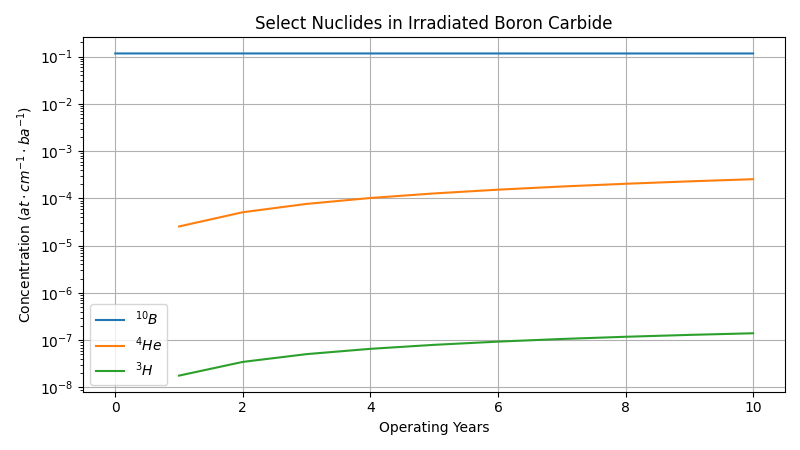
\includegraphics[width=0.9\textwidth]{./Plotter/boronburn/AtomDens}
    \caption[\acs{msnb} Irradiated Boron Carbide]{Concentration of tritium, helium-4, and boron-10 in irradiated boron carbide during a decade-long \acs{msnb} deployment.}
    \label{fig:BoronBurn}
\end{figure}

After 100 MW-yr of heat output, just 0.22\% of the \B[10] was consumed. This caused a negligible effect on the reactivity worth of each control drum. In addition to the deactivation of the neutron poison itself, two gases of interest are formed in boron carbide under neutron fluence. Helium-4 is formed after the alpha particle from the primary capture reaction is de-ionized:

\begin{reaction} \label{rxn:B10cap}
    ^{10}B + n \to {^{7}Li} + \alpha
\end{reaction}

By the end of the decade scale operation, 58 moles of helium have been formed by this pathway. This is a significant amount that will need to be off-gassed operation, and could cause swelling if the material is not properly qualified. Tritium is also formed both directly and indirectly by the $^{10}B(n,2\alpha){^{3}H}$ and $^{7}Li(n,n\alpha){^{3}H}$ reactions. At the end of the study, the control material of the \acs{msnb} contained 31.9 millimoles, or 95.7 mg of tritium. This will account for a small amount of the total radioactivity in the decommissioned \acs{msnb}.

\subsection{Neutron Spectra}
A detector code was used to study the volume average neutron flux in three concentric regions. A material detector card was specified for:
\begin{enumerate*}
    \item the molten salt in the core;
    \item the reflector; and
    \item the molten salt in the downcomer.
\end{enumerate*}
500 energy bins of equal lethargy\footnote{Neutron lethargy is a logarithmic energy ratio. Energy bins of equal lethargy width are uniformly distributed when plotted on a log-axis.} width from 10 $\mu$eV to 20 MeV. Figure \ref{fig:Spectrum} displays the neutron spectra in the three regions within the \acs{msnb}.

\begin{figure}[ht!]
    \centering
    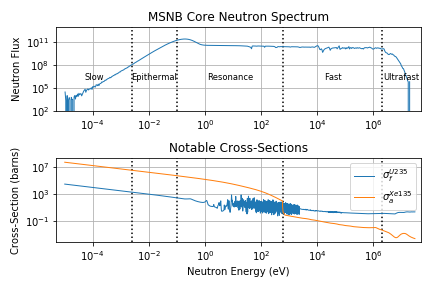
\includegraphics[width=0.9\textwidth]{./Plotter/Detector/Spectrum}
    \caption[\acs{msnb} Neutron Energy Spectrum]{\raggedright \acs{msnb} neutron energy spectrum in core, reflector, and downcomer.}
    \label{fig:Spectrum}
\end{figure}

The \acs{msnb} is a fast/epithermal reactor. Most fission neutrons that are emitted at ~2 MeV are not fully thermalized, as they are in \acsp{lwr}. Within the core, The volume average flux generally diminishes as the neutron energy drops, with some discontinuities caused by major resonance peaks of \F, \Li[7], \Na, \K, \U[235], and \U[238], the major constituents of the molten salt fuel. For most neutron energies, the volume average flux in the downcomer is about 2 orders of magnitude, indicating leakage of approximately 1\%. 

An epithermal peak of about 0.1 eV is observed in the downcomer and reflector. The corresponding peak is much smaller in the core spectrum. This implies that this design is not optimally moderating neutrons in the core, \ie the lower energy neutrons have small path length inside the core. This is likely because those neutrons that transport to the edge of the core, are slowed in the reflector, and re-enter the core do not penetrate deep into the core before inducing fission or being captured. Because the \acs{msnb} has ample shut-down margin and limited excess reactivity, it is recommended that in future work, a wider diameter core with smaller flow paths surrounded by in-pile moderation is designed. This will allow the core to make better use of the epithermal peak that is caused by the beryllium oxide reflector, increase the overall macroscopic fission cross-section, and produce a more reactive core.


\subsection{Actuator Curve}\label{sec:actuator}

\begin{figure}[!ht]
    \centering
    \subfloat[\centering Xenon-135 Build-up]{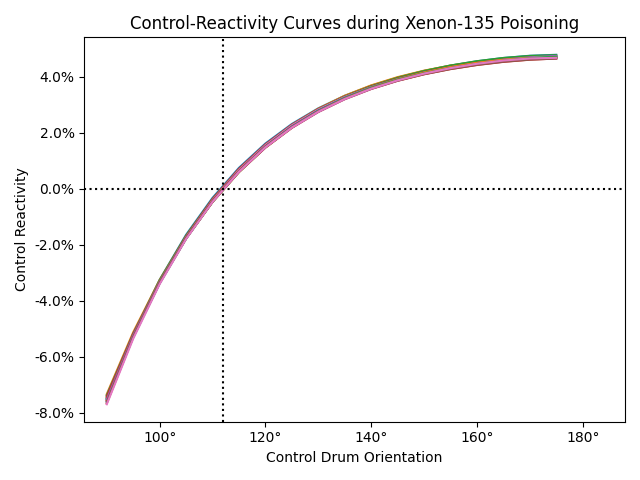
\includegraphics[width=0.49\textwidth]{/CurveFits/eqXe}}
    \subfloat[\centering Depletion]{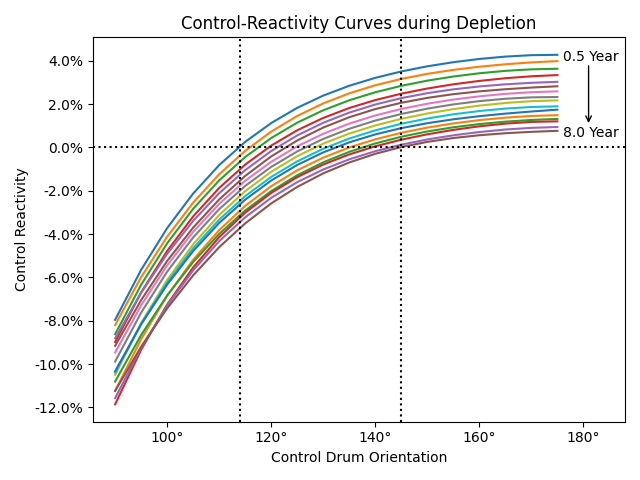
\includegraphics[width=0.49\textwidth]{/CurveFits/depletion}}
    \caption[Control Reactivity Curve]{Control drum angle vs. reactivity curves. Each curve corresponds to a different burn-up level:
    \begin{enumerate*}[label=\alph*)]
        \item 6 hour increments until \Xe reaches equilibrium`'; and 
        \item 6 month increments until the fuel is depleted enough that the \acs{msnb} has very little excess reactivity; 
    \end{enumerate*}
    }
    \label{fig:ControlReactivityCurve}
\end{figure}

The controller that is tuned and studied in Section \ref{sec:simulation} depends on a detailed actuator characterization. The \acs{msnb}'s static response to the orientation of the control drums were studied over the life of the reactor in an alternating methodology of criticality and burn-up modeling, detailed in Section \ref{Section:Serpent}. Figure \ref{fig:ControlReactivityCurve} depicts the evolution of the core reactivity vs. the rotational angle of the control drum as the \Xe level rises to equilibrium, and as the \U[235] is depleted. The controller model treats the control drum as an \acs{lti} system. The figure clearly shows that the actuator response is neither linear nor time-invariant. Over time, the reactor's response to the actuator changes, however, these are not rapid changes; the \Xe worth at equilibrium for the specific power of study (10 MW) is small enough that the curves overlap, with only dozens of pcm separating the fresh and poisoned fuel. Furthermore it takes eight years for the unity point to drift by approximately 20 degrees. The evolution of the actuator response can easily be modeled using a look-up table. The controller will set a different bias and use a different gain depending on the length of time that the \acs{msnb} has operated. The data was fit to a series of fourth order polynomials which the process simulator can use to calculate the control reactivity ($\rho$) given the control drum orientation ($\theta$):

\begin{equation}
    \rho = c_0 + c_1\theta + c_2\theta^2 + c_3\theta^3 + c_4\theta^4
\end{equation}

During normal operation, the reactor will only be made slightly supercritical to power up or subcritical to power down, likely on the order of tens to hundreds of pcm. This corresponds to a small rotation of the control drums. For the purposes of controller design, the control-reactivity curve can be linearized simply by solving for the root of the polynomial and computing the derivative at that point. The root of the curve corresponding to the current depth of burn-up will be set as the controller bias, while the slope of the tangent line (in pcm/degree) can be used to scale the controller gain (in degree/kW) and obtain the desired combined controller-actuator gain (in pcm/kW). Notably, the root of all of the curves lies above its inflection point. As a result the actuator will insert less positive reactivity than the controller intends during an up-transient, land more negative reactivity than the controller intends during a down-transient. The deviation between the polynomial and linearization is small for the expected range of control drum orientations, but this may result in slightly better performance when increasing the power duty. The polynomial coefficients defining the curves and root/tangent slope are listed in Tables \ref{tab:Xefit} and \ref{tab:Depletionfit}. $c_0$ could be adjusted to account for a different operating temperature, which would shift the curve up or down according to $\alpha_t$, and require re-linearization around the new root. 

\begin{table}[t!]
    \caption[Control Reactivity Curve Fit - Equilibrium Poisoning]{Polynomial coefficients, root, and slope for the control drum vs. reactivity curves during equilibrium poisoning.}
    \centering\begin{tabular}{c|ccccc|cc}
    \hline
    Hours & c\textsubscript{4} \sci[9] & c\textsubscript{3} \sci[6] & c\textsubscript{2} \sci[4] & c\textsubscript{1} \sci[2] & c\textsubscript{0} & root ($^o$) & slope ($pcm/^o$) \\ \hline
    0  & -2.797 & 1.789 & -4.361 & 4.829 & -2.009 & 111.41 & 224.24 \\
    6  & -2.076 & 1.372 & -3.475 & 4.005 & -1.727 & 111.71 & 221.35 \\
    12 & -2.701 & 1.725 & -4.211 & 4.676 & -1.953 & 111.61 & 221.89 \\
    18 & -2.780 & 1.797 & -4.393 & 4.874 & -2.031 & 111.63 & 224.23 \\
    24 & -2.292 & 1.501 & -3.753 & 4.265 & -1.817 & 111.97 & 218.62 \\\hline
    30 & -2.226 & 1.470 & -3.706 & 4.244 & -1.819 & 111.94 & 222.27 \\
    36 & -2.116 & 1.424 & -3.643 & 4.211 & -1.814 & 111.77 & 223.04 \\
    42 & -2.086 & 1.376 & -3.483 & 4.009 & -1.728 & 112.02 & 217.91 \\
    48 & -2.330 & 1.517 & -3.776 & 4.277 & -1.819 & 112.09 & 217.58 \\\hline
    54 & -2.174 & 1.439 & -3.635 & 4.168 & -1.788 & 112.04 & 219.12 \\
    60 & -2.287 & 1.508 & -3.797 & 4.334 & -1.851 & 111.96 & 221.58 \\
    66 & -2.696 & 1.716 & -4.178 & 4.636 & -1.937 & 112.00 & 218.60 \\
    72 & -1.990 & 1.332 & -3.406 & 3.951 & -1.712 & 112.08 & 217.56 \\\hline
    78 & -2.227 & 1.464 & -3.674 & 4.190 & -1.791 & 112.07 & 216.57 \\
    84 & -2.665 & 1.704 & -4.162 & 4.626 & -1.935 & 111.98 & 217.40 \\
    90 & -2.627 & 1.696 & -4.177 & 4.668 & -1.958 & 111.88 & 220.09 \\
    96 & -2.859 & 1.818 & -4.413 & 4.870 & -2.023 & 112.05 & 219.42 \\
    \end{tabular}
    \label{tab:Xefit}
\end{table}

\begin{table}[bh!]
    \caption[Control Reactivity Curve Fit - Fuel Depletion]{Polynomial coefficients, root, and slope for the control drum vs. reactivity curves during fuel depletion.}
    \centering\begin{tabular}{c|ccccc|cc}
    \hline
    Years & c\textsubscript{4} \sci[9] & c\textsubscript{3} \sci[6] & c\textsubscript{2} \sci[4] & c\textsubscript{1} \sci[2] & c\textsubscript{0} & root ($^o$) & slope ($pcm/^o$) \\ \hline
    0.0 & -2.797 & 1.789 & -4.361 & 4.829 & -2.009 & 111.41 & 224.24 \\
    0.5 & -2.755 & 1.755 & -4.272 & 4.732 & -1.976 & 113.69 & 203.69 \\
    1.0 & -1.838 & 1.253 & -3.253 & 3.826 & -1.682 & 115.79 & 189.71 \\
    1.5 & -2.533 & 1.632 & -3.253 & 4.507 & -1.909 & 117.38 & 175.96 \\
    2.0 & -2.418 & 1.578 & -3.930 & 4.440 & -1.895 & 119.45 & 161.06 \\\hline
    2.5 & -1.461 & 1.026 & -2.750 & 3.337 & -1.515 & 121.06 & 152.71 \\
    3.0 & -1.137 & 0.856 & -2.425 & 3.070 & -1.440 & 122.67 & 146.08 \\
    3.5 & -2.054 & 1.357 & -3.433 & 3.953 & -1.727 & 124.58 & 130.85 \\
    4.0 & -2.527 & 1.617 & -3.967 & 4.438 & -1.892 & 126.46 & 120.67 \\\hline
    4.5 & -2.869 & 1.831 & -4.460 & 4.935 & -2.081 & 128.35 & 111.30 \\
    5.0 & -2.338 & 1.520 & -3.785 & 4.291 & -1.855 & 130.55 & 102.04 \\
    5.5 & -1.471 & 1.054 & -2.852 & 3.467 & -1.585 & 132.29 & 93.34 \\
    6.0 & -2.626 & 1.702 & -4.211 & 4.729 & -2.027 & 134.96 & 83.90 \\\hline
    6.5 & -1.672 & 1.141 & -2.985 & 3.550 & -1.607 & 137.45 & 77.56 \\
    7.0 & -3.321 & 2.095 & -5.036 & 5.492 & -2.292 & 139.19 & 69.73 \\
    7.5 & -2.419 & 1.579 & -3.936 & 4.459 & -1.932 & 142.69 & 59.45 \\
    8.0 & -7.991 & 0.648 & -1.960 & 2.623 & -1.305 & 144.62 & 55.65 \\
    \end{tabular}
    \label{tab:Depletionfit}
\end{table}

\section{Multi-physics Simulation}\label{sec:simulation}

\subsection{Steady-State}

\begin{figure}[ht!]
    \centering
    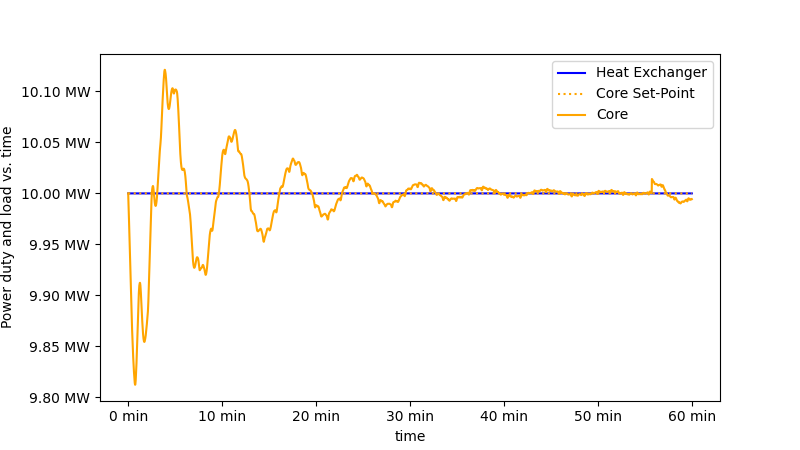
\includegraphics[width=0.9\textwidth]{Simulator/SteadyState/t_vs_Qt}
    \caption[Steady state power response]{Core power response to a steady heat exchanger demand of 10 MW given the initial conditions.}
    \label{fig:SS-Power}
\end{figure}

\begin{figure}[ht!]
    \centering
    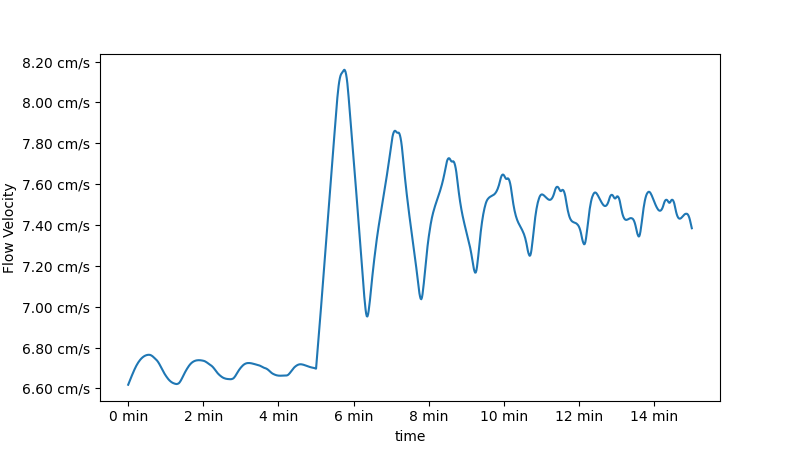
\includegraphics[width=0.9\textwidth]{Simulator/SteadyState/t_vs_velocity}
    \caption[Steady state velocity response]{Core velocity response to a steady heat exchanger demand of 10 MW given the initial conditions.}
    \label{fig:SS-Velocity}
\end{figure}

\subsection{Up-Step}

\subsubsection{Autonomous Response}


\subsubsection{Controller Tuning}


\subsubsection{Controller Response}


\subsection{Down-Step}

\subsection{Start-Up}

\subsection{Shut-Down}

\subsection{Demand-Response}